\documentclass[12pt,letterpaper]{article}
\usepackage[utf8]{inputenc}
\usepackage{amsmath,amsthm,amsfonts,amssymb,amscd}
\usepackage[table]{xcolor}
\usepackage[margin=2.5cm]{geometry}
\usepackage{ragged2e}
\usepackage{graphicx}
\usepackage{multicol}
\newlength{\tabcont}
\setlength{\parindent}{0.0in}
\setlength{\parskip}{0.05in}

\begin{document}
	
	\large \textbf{Nome}: Luís Felipe de Melo Costa Silva \\
	\textbf{Número USP}: 9297961 
    
	\begin{center}
		\LARGE \bf
		Lista de Exercícios 1 - MAC0444
	\end{center}
	
	\section*{Exercício 1}
	
	\textbf{a)} Para esta sentença, usaremos o conjunto $S$ = \{pedra, papel, tesoura\}, e o predicado que usaremos será $P(x,y)$ = $x$ não perde de $y$, (para $x \in S$ e $y \in S$) nas regras do Jokenpô. Aqui, não perder significa ganhar ou empatar. Com isso, teremos que:
	
	1. $\forall x \forall y \forall z((P(x,y)\land P(y,z)) \to P(x, z))$ será falsa, com x = pedra, y = tesoura e z = papel.
	
	2. $\forall x \forall y((P(x,y) \land P (y,x)) \to x=y)$ será verdadeira, pois se $x$ não perde de $y$ e $y$ não perde de $x$, nas regras do Jokenpô, isso significa que $x=y$.
	
	3. $\forall x\forall y(P(a,y) \to P(x,b))$ será verdadeira, desde fixemos $a = b$.\\
	
	\textbf{b)} O predicado usado aqui será P(x,y) = x e y são pares, e o conjunto de números usados será o dos naturais. Com isso:
	
	1. $\forall x \forall y \forall z((P(x,y)\land P(y,z)) \to P(x, z))$ será verdadeira, pois se $x$ e $y$ são pares, e $y$ e $z$ são pares, então $x$ e $z$ são pares.
	
	2. $\forall x \forall y((P(x,y) \land P (y,x)) \to x=y)$ será falsa, pois mesmo que $x$ e $y$ sejam pares, eles não precisam ser necessariamente iguais.
		
	3. $\forall x\forall y(P(a,y) \to P(x,b))$ será verdadeira, desde fixemos $a$ como um número ímpar.\\
	
	\textbf{c)} Nessa sentença, o predicado usado será $P(x,y)$ = $x \leq y$, no conjunto dos Racionais.
	
	1. $\forall x \forall y \forall z((P(x,y)\land P(y,z)) \to P(x, z))$ será verdadeira, e isso sai da definição de Racionais.
	
	2. $\forall x \forall y((P(x,y) \land P (y,x)) \to x=y)$ será verdadeira, de maneira análoga ao item anterior.
	
	3. $\forall x\forall y(P(a,y) \to P(x,b))$ será falsa, desde fixemos $a$ e $b$ como o menor número racional existente.
	
	\section*{Exercício 2}
		
	\textbf{a)} A nossa base de conhecimento será composta por:
	\begin{multicols}{2}
		\begin{itemize}
			\item $\forall x (\lnot E(x)\to A(x))$
			\item $\forall x (A(x)\to \lnot G(c,x))$
			\item $\forall x (\lnot G(x,n)\to\lnot E(x))$
			\item $\forall x (G(T,x)\to\lnot G(M,x))$
			\item $\forall x (\lnot G(T,x)\to G(M,x))$
			\item $G(T,c) \land G(T,n)$
		\end{itemize}
	\end{multicols}
	
	
	Onde:
	
	\begin{itemize}
		\item $E(x)$ significa que $x$ é um esquiador.
		\item $A(x)$ significa que $x$ é um alpinista.
		\item $G(x,y)$ significa que $x$ gosta de $y$.
		\item $T$ é Tony, $M$ é Mike e $J$ é John.
		\item $c$ é chuva e $n$ é neve.
		\item Os predicados se aplicam apenas aos membros do Clube Alpino
	\end{itemize}
	
	Também sabemos que Tony, Mike, John $\in ClubeAlpino$.\\
	
	\textbf{b)} Queremos provar que KB $\vdash \exists x (A(x) \land \lnot E(x))$.
	
	\begin{enumerate}
		\item Sabemos que $\forall x (G(T,x)\to\lnot G(M,x))$.
		\item Seja $x = n$. Temos que $G(T,n)$, portanto, 	$\lnot G(M,n)$.
		\item Como $\forall x (\lnot G(x,n)\to\lnot E(x))$, podemos inferir que $\lnot E(M)$.
		\item Já que  $\forall x (\lnot E(x)\to A(x))$, então	$A(M)$. \qed
	\end{enumerate}
	
	\textbf{c)} Sem a informação que $\forall x (G(\text{Tony},x)\to\lnot G(\text{Mike},x))$, é impossível fazer a prova acima, já que ela se inicia com esse conhecimento. Sabemos que Tony gosta de neve, e não conseguiremos mostrar que Mike não gosta de Neve. \\
	
	\textbf{d)} Para usar a resolução, teremos que transformar nossa KB na Forma Normal Conjuntiva:
	
	\begin{multicols}{2}
		\begin{itemize}
			\item $\forall x (E(x)\lor A(x))$
			\item $\forall x (\lnot A(x)\lor \lnot G(c,x))$
			\item $\forall x ( G(x,n)\lor\lnot E(x))$
			\item $\forall x (\lnot G(T,x)\lor\lnot  G(M,x))$
			\item $\forall x (G(T,x)\lor G(M,x))$
			\item $G(T,c)$
			\item $G(T,n)$
		\end{itemize}
	\end{multicols}
	
	Iremos mostrar que $\exists x (A(x) \land \lnot E(x))$. Para resolver com extração de memória, vamos adicionar um predicado de resposta ao que queremos provar, logo, $\exists x [(A(x) \land \lnot E(x)) \land R(x)]$. Com isso, teremos a cláusula $[\lnot A(x), E(x), R(x)]$. Então:
	
	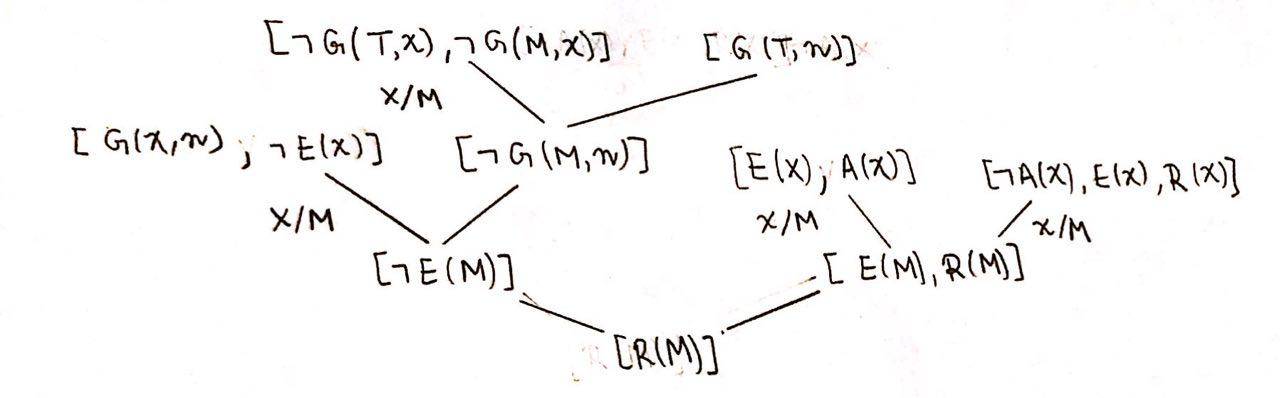
\includegraphics[width=\textwidth]{2d.jpg}
	
	Portanto, a resposta é Mike.
			 
\end{document}